\subsection{Batch K-means}

\mode<presentation>{
\begin{frame} 
    \begin{center} \huge
        \subsecname
    \end{center}
    \begin{center}
		Use all data points at every iteration.
    \end{center}
\end{frame}
}

\subsubsection{Algorithm overview}

\begin{frame}{\subsecname:~\subsubsecname}

\notesonly{
The way we've approached previous optimization problems is to derive how the parameters are updated to minimize the cost function and then we look at the algorithm that make use of the derived update rules to find a solution to the problem. Given the simplicity of the K-means algorithm, we will opt to first look at the algorihtm that implements K-means to understand how it operates and interesting aspects of the solution that it finds. We will then follow this by discussing the derivations we encountered in the algorithm (e.g. the update rule)

\underline{How does K-means work?} 
}

An iterative two-step procedure after initializing $\big\{ \vec{w}_q \big\}$:
\begin{enumerate}
\item \textbf{assign} each point to its \emph{nearest} prtototype (nearest $\corresponds$ smallest Euclidiean distance.)
\item \textbf{update} all cluster prototypes by moving them to their cluster's center of mass.
\end{enumerate}

\end{frame}

\subsubsection{Algorithm details}

\begin{frame}{\subsecname:~\subsubsecname}

\vspace{-0.4cm}
\begin{figure}[!th]
\footnotesize
\removelatexerror
\begin{algorithm}[H]
\DontPrintSemicolon
  random initialization of prototypes, e.g.\ $\vec{w}_{q} = \langle \vec{x} \rangle +\vec{\eta}_{q}, \hspace{0.2cm} \vec{\eta}_{q}  \text{ small random vector}$\;
  \Begin(loop){
  (1) choose  $m_q^{(\alpha)}$ such that $E^T$ is minimal for the given prototypes\;
\[ m_q^{(\alpha)} = \left\{ \begin{array}{ll}
	1, & \text{if } q = \argmin_{\gamma} \big| \vec{x}^{(\alpha)}
		- \vec{w}_{\gamma} \big| \\
	0, & \text{else}
\end{array} \right. \]
$\Rightarrow$ assign \textbf{every} data point to its nearest prototype \;
\;
(2) choose  $\vec{w}_q$ such that $E^T$ is minimal for the \textbf{new} assignments\;
\[ \vec{w}_q = \frac{\sum\limits_{\alpha} m_q^{(\alpha)} \vec{x}^{(\alpha)}}{
	\sum\limits_{\alpha} m_q^{(\alpha)}}
\]
$\Rightarrow$ set $\vec{w}_q$ to the center of mass of its assigned data
}
    \label{alg:batch-k-means}
    \caption{batch K-means}
\end{algorithm}
\end{figure}
\end{frame}

\notesonly{
The steps for finding the optimal prototype locations and assignments are described in Algorithm \ref{alg:batch-k-means}.
It is important to understand that a single iteration, takes \textbf{all} points into account. This is not a loop that iterates over the individual points. Each iteration deals with assignment of \textbf{all} points and updating the location of the prototypes considering all data points collectively within that iteration.
The stopping criterion for the batch K-means algorithm\ref{alg:batch-k-means}, i.e. when to stop the loop, can be chosen by detecting that the location of prototypes are no longer moving. Alternatively, one could keep track of the difference in the value of $E^T$ between two successive iterations until it reaches some desired threshold.
}
 
\begin{frame}
Things to note about \emph{batch K-means}:

\begin{enumerate}
\item $E^T$ is \emph{non-increasing}\footnote{Non-increasing $\corresponds$ decreasing OR unchanged.}. We either move to an improved solution with lower cost or the cost remains unchanged.
\item This is a nonconvex optimization problem. This means that we may arrive at local optima which yield bad solutions.
\item \notesonly{Additionally, }the global minimum is not unique. There exist $M! = \prod_{i=1}^{M} i$ different assignments with the same lowest cost. This is a result of permutation symmetry. \notesonly{If we suddenly start labeling all points assigned to cluster $4 \rightarrow 7$, and simultaneously label all points originally assigned to $7 \rightarrow 4$, the cost remains unchanged.}
The algorithm is indifferent to the index value of a cluster. The cluster indices are simply ``names''\notesonly{ to differntiate between the clusters and changing their names does not alter the solution obtained}.
\begin{center}
\begin{minipage}{0.45\textwidth}
	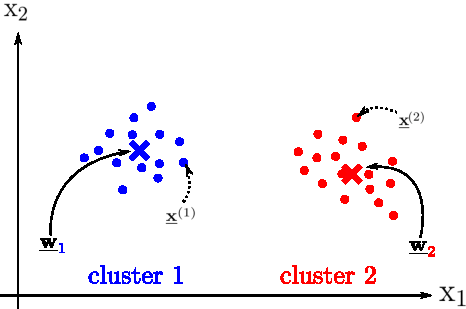
\includegraphics[width=0.8\textwidth]{img/clustering_color_proto}
\end{minipage}
\begin{minipage}{0.45\textwidth}
	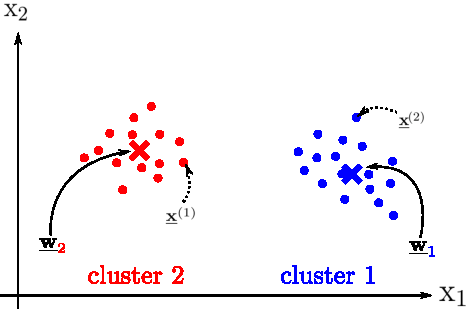
\includegraphics[width=0.8\textwidth]{img/clustering_color_proto_swap}
\end{minipage}
\captionof{figure}{Two clustering solutions with equal cost}
\end{center}
 
\end{enumerate}

\end{frame}

\begin{frame}

\question{How is K-means an optimziation algorithm?}

\slidesonly{
\begin{center}
	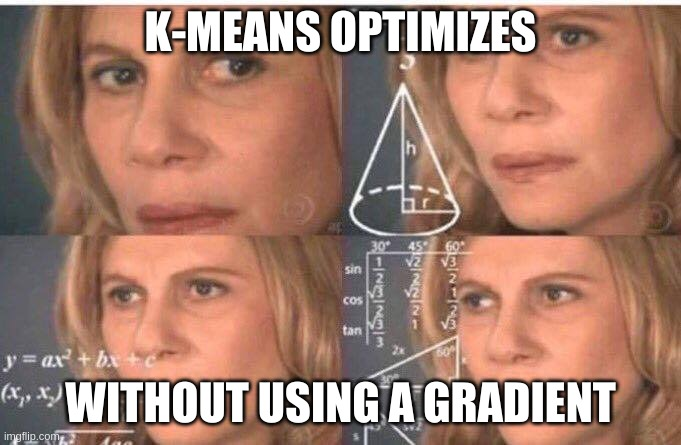
\includegraphics[width=0.3\textwidth]{img/meme_kmeansoptimizes}
\end{center}
}

\slidesonly{
Updating the protptypes by $\vec{w}_q = \frac{\sum\limits_{\alpha} m_q^{(\alpha)}
		\vec{x}^{(\alpha)}}{\sum\limits_{\alpha} m_q^{(\alpha)}}$ minimizes $E^T$.
We just have to find the gradient.
}

\notesonly{
We've seen how one would implement K-means. More specifically, we've seen that the prototypes $\vec w_q$ are updated every iteration such that they represent the mean of the points assigned to them in that iteration. However, we have yet to show that this iterative method effecitvley minimizes $E^T$. We do so by evaluating the gradient, finding the zero-crossing. We are effectively looking for the extrema of the cost function $E^T$.
}

\end{frame}

\notesonly{
Recall the definition for the cost function:
}

\begin{frame}{K-means really does optimize}
\begin{equation}
E_{ \big[ \big\{ m_q^{(\alpha)} \big\}, \big\{ \vec{w}_q \big\} 
		\big] }^T = \frac{1}{p} \sum\limits_{q,\alpha} m_q^{(\alpha)}
		\big( \vec{x}^{(\alpha)} - \vec{w}_q \big)^2 \eqexcl 
		%\min
		\underset{\big\{ m_q^{(\alpha)} \big\}, \big\{ \vec{w}_q \big\}}{\min}
\end{equation}

The condition for an extremum is as follows:
\begin{align}
	\frac{\partial}{\partial \vec{w}_q} E^T
	&=
	\frac{\partial}{\partial \vec{w}_q} \bigg\{ \frac{1}{p} 
	\sum\limits_{q', \, \alpha} m_{q^{'}}^{(\alpha)} 
	\big( \vec{x}^{(\alpha)} - \vec{w}_{q^{'}} \big)^2 \bigg\} \\
	& = -\frac{2}{p} \sum_{\alpha=1}^{p} m_q^{(\alpha)} 
		\big( \vec{x}^{(\alpha)} - \vec{w}_q \big) \eqexcl 0
\end{align}
\slidesonly{

Solve for $\vec w_q$...
}

\end{frame}
\begin{frame}

Solve for $\vec w_q$:


\begin{align}
 -\frac{2}{p} \sum\limits_{\alpha} m_q^{(\alpha)} 
		\big( \vec{x}^{(\alpha)} - \vec{w}_q \big) &= 0 \quad (\text{\small omit the constant}\; -2/p),\\
 \sum\limits_{\alpha} m_q^{(\alpha)} 
		\big( \vec{x}^{(\alpha)} - \vec{w}_q \big) &= 0\\
 \sum\limits_{\alpha} m_q^{(\alpha)} 
		\vec{x}^{(\alpha)} &= \sum\limits_{\alpha} m_q^{(\alpha)} \vec{w}_q \\
		\vec w_q \;\text{\small does not depend on}\; &\alpha, \;\text{\small use $\sum\limits_{\alpha} m_q^{(\alpha)}$ as a normalization factor},\\
	\leadsto \vec{w}_q &= \frac{\sum\limits_{\alpha} m_q^{(\alpha)}
		\vec{x}^{(\alpha)}}{\sum\limits_{\alpha} m_q^{(\alpha)}}
\end{align}

\end{frame}
\begin{frame}

\slidesonly{
$$
	\leadsto \vec{w}_q = \frac{\sum\limits_{\alpha} m_q^{(\alpha)}
		\vec{x}^{(\alpha)}}{\sum\limits_{\alpha} m_q^{(\alpha)}} \qquad \text{(extremum found)}
$$
}
\notesonly{Now we've found the extremum. }We still need to identify if this corresponds to a maximum or minimum.


The condition for a minimum is that the second-order partial derivatives, the \emph{Hessian}, is positive:

\begin{align}
	\frac{\partial^2}{\partial \mathrm{w}_{qi} \partial \mathrm{w}_{
			q'j}} \big\{ E^T\big\}
	&=
		\frac{\partial^2}{\partial \mathrm{w}_{qi} \partial \mathrm{w}_{
			q'j}} \bigg\{ \frac{1}{p} \sum\limits_{q^{''}, \alpha}
			m_{q^{''}}^{(\alpha)} \big( \vec{x}^{(\alpha)} - \vec{w}_{q^{''}}
			\big)^2 \bigg\} \\
		& = \frac{\partial}{\partial \mathrm{w}_{q^{'}j}} \bigg\{
			-\frac{2}{p} \sum\limits_{\alpha} m_q^{(\alpha)} 
			\big( \mathrm{x}_i^{(\alpha)} - (\vec{w})_{qi}
			\big) \bigg\} \\
\notesonly{
		& = \left( \frac{2}{p} \sum\limits_{\alpha} m_q^{(\alpha)} \right)
			\delta_{ij} \delta_{qq^{'}}
			}
\end{align}
\end{frame}

\begin{frame}
\slidesonly{
\begin{align}
	\frac{\partial^2}{\partial \mathrm{w}_{qi} \partial \mathrm{w}_{
			q'j}} \big\{ E^T\big\}
	&=
		\frac{\partial^2}{\partial \mathrm{w}_{qi} \partial \mathrm{w}_{
			q'j}} \bigg\{ \frac{1}{p} \sum\limits_{q^{''}, \alpha}
			m_{q^{''}}^{(\alpha)} \big( \vec{x}^{(\alpha)} - \vec{w}_{q^{''}}
			\big)^2 \bigg\} \\
		& = \frac{\partial}{\partial \mathrm{w}_{q^{'}j}} \bigg\{
			-\frac{2}{p} \sum\limits_{\alpha} m_q^{(\alpha)} 
			\big( \mathrm{x}_i^{(\alpha)} - (\vec{w})_{qi}
			\big) \bigg\} \\
		& = \left( \frac{2}{p} \sum\limits_{\alpha} m_q^{(\alpha)} \right)
			\delta_{ij} \delta_{qq^{'}}
\end{align}
}

where $\delta_{ij}$ and $\delta_{qq^{'}}$ are the dirac-delta functions ($\delta_{ij}=1$ iff $i=j$ and $=0$ otherwise). 
Since $\frac{2}{p} \sum\limits_{\alpha} m_q^{(\alpha)}$ is always positive \notesonly{(c.f. \eqref{eq:assignmentnormalization})}:

\begin{itemize}
	 \itR The Hessian is a diagonal matrix with all positive entries $\,\to\,$ condition for minimum is always satisfied.
	 \itR however: minimizing $E^{T}$ is not a convex optimization problem (because of the combination of steps 1 and 2).
\end{itemize} 

\end{frame}

% --------------------------------------------------------------------------
\begin{frame} \frametitle{Interpreting the solution}
\begin{figure}[h]
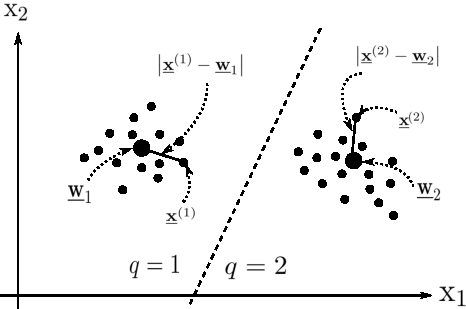
\includegraphics[width=5.0cm]{img/section4_fig2_withincluster}
\end{figure}
$$
	E_{ \big[ \big\{ m_q^{(\alpha)} \big\}, \big\{ \vec{w}_q \big\} 
		\big] }^T = \frac{1}{p} \sum\limits_{q,\alpha} m_q^{(\alpha)}
		\big( \vec{x}^{(\alpha)} - \vec{w}_q \big)^2
$$
\begin{itemize}
 \itR If $\vec{w}_q$ is center of mass $\implies$ $E^T = \mathrm{variance}$.
 \itR $E^T$ is non-increasing in every step and $E^T$ is bounded from below \\ $\,\to\,$ K-means clustering converges to a (local) optimum of $E^T$. 
\itR $E^T$ at the solution can be interpreted as the ``size'' (variance) of the clusters.
\end{itemize} 
\end{frame}

